\documentclass[12pt]{article}
\usepackage[english]{babel}
\usepackage{graphicx}
\usepackage{tabularx}
\usepackage[backend=bibtex, natbib=true]{biblatex}
\usepackage{listings}
\usepackage{placeins}
\setlength{\parindent}{0pt}

\bibliography{bibliography}
%opening
%Here you can enter your names and titleof your report
\title{HIS SSNS - Bi-Weekly Report 4}
\author{
	 Raul Bertone
\and Elis Harruni
\and Muyassar Kokhkharova
\and Saidar Ramazanov
\and Xhoni Robo
}

\begin{document}

\maketitle

%The abstract is used to give a short overview of your report, article, ...
\begin{abstract}
 This report covers the progress made by the group on their project during the time period 15th to the 28th of June 2018. Individual and total group effort is at the end of this report.
\end{abstract}

\section{Sensortag}
During testing of the Sensortag, a bug was encountered: every few seconds the data stream coming from the Sensortag would freeze, only to resume after approximately one second. Additionally, after the first pause, the values measured by the accelerometer would be off by a factor of 2. This behavior was present both while the Sensortag was connected to a smartphone as well as to the Launchpad. This pointed to the problem being in the modification that we performed in the Sensortag’s code.\\\\
After talking with Group 2, which made similar modifications but didn’t use the “EXCLUDE” directives for the pre-processor, we were mislead into thinking that the directives themselves were at fault. This made us lose some time chasing a red herring. Debugging revealed however that the “bug” was actually a feature we inadvertently turned on, namely  Wake-On-Motion. This interrupts the sending of sensor data when there is no movement for more than a few seconds. Turning the feature back off, neatly solved the problem.

\section{Fall Notification Service}
We developed the last main missing feature, the service that handles the notifications triggered by the detection of a fall. Its code interacts with each and every other part of the desktop application and ties them all together.\\
On start the FNS idles while waiting for a trigger. When the fall detection algorithm thinks the user has fallen, it alerts the FNS which turns on the buzzer in the Sensortag and raises the “Fall Detected” flag in the GUI and then waits for a preset amount of time (default 10 seconds) for feedback from the user in the form of a button press on the Sensortag. If no such feedback comes, help is requested (an email is sent to the helper’s address) and the “Help Requested” flag is raised in the GUI. Instead, in case a button is pressed before the preset time has elapsed, the buzzer is turned off and the “Fall Detected” flag lowered, after which the cycle repeats itself.
Below you see a state machine diagram illustrating the service’s operation:

\FloatBarrier
\begin{figure}[h]
	\centering
	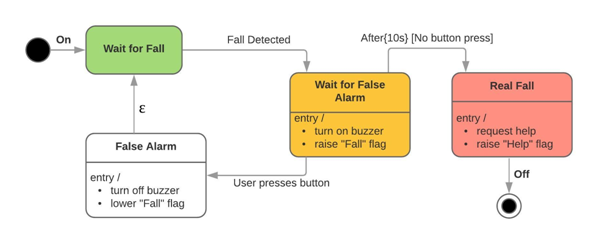
\includegraphics[scale=0.80]{images/State_Diag.png}
	\caption{State Diagram}
	\label{img:State_Diag}
\end{figure}
\FloatBarrier

As part of the development of this feature, we also collaborated to link it to the GUI. In particular Raul explained in detail the Fall Notification Service to Muyassar Kohkhkarova, so that she could modify it to interact with the GUI for turning the necessary flags on and off.\\

\section{Bringing the Application Together}
So far the members of the team have each worked on one of the big components of the application. Now that these parts are complete, in order to have a fully working application, they must be brought together and connected to each other.

\subsection{Desktop Application Improvements}
Our application until now was completely separated the front end and back end.\\
The GUI part was a dummy without functionalities, and the logic was already a console application.
This two weeks we have developed the back end more as can be seen from the UML. Also, we started to implement the Controllers that do the connection between the model that was already the console Application we used for getting data and test our algorithm and also made some changes to the GUI.

\FloatBarrier
\begin{figure}[h]
	\centering
	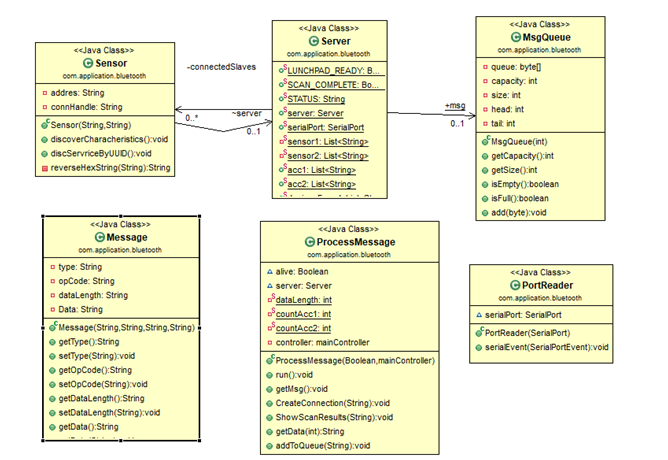
\includegraphics[scale=0.72]{images/UML_1.png}
	\caption{UML Backend Diagram}
	\label{img:UML_1}
\end{figure}
\FloatBarrier

We have also made progress on defining the right bit mask for the services to help on communication
between our application and Launchpad and its slaves.\\
As can be seen in the UML we have created a new Class now called sensor and we create a new instance of that class whenever we establish a new connection between server(central device lunchpad) and a slave, in this case the Sensor. That helps because now after we discover Services and Characteristics, we can save them into that instance. After that we can create every kind of what can be called commands but are actually hexadecimal strings sent to the Launchpad by the serial port, since every instance will have its Characteristics and the connection handles every detail about the slave. The class called Server contains a collection of the connected slaves and can do whatever it wants with those.\\
The problems that we am facing now are the buzzer service and the button service because we have to find the right hex values for them and to create the bit mask for the Launchpad.

\section{GUI Updates}
On top of the buttons, a ListBox was added to allow the user to select
the desired Sensortags to be connected. While this works as intended most
of the time, some problems arise when there are multiple devices around the
launchpad that have Bluetooth open. While they do not get recognized by
the application, and thus are not allowed to connect, the scanning function
finds only 8 devices at a time and currently these devices are not only the
Sensortags. It happens that either one or both Sensortags are not in the list
of scanned devices. This issue is currently a high priority that will be fixed
before the final report.

\FloatBarrier
\begin{figure}[h]
	\centering
	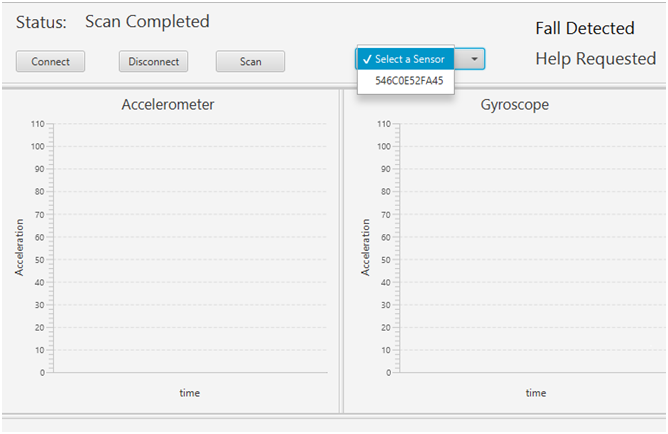
\includegraphics[scale=0.80]{images/UI_4.png}
	\caption{Current GUI}
	\label{img:UI_4}
\end{figure}
\FloatBarrier

\subsection{Changing Label Colors in GUI}
In mainController we set a reference to mainController so that the FallNotificationService can change the color of the labels.
\FloatBarrier
\begin{figure}[h]
	\centering
	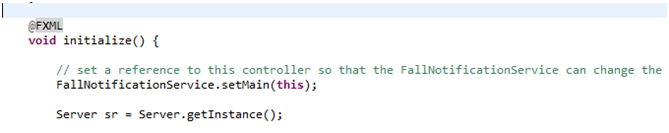
\includegraphics[scale=0.80]{images/UI_1.png}
	\caption{mainController Reference}
	\label{img:UI_1}
\end{figure}
\FloatBarrier
\clearpage
In FallNotificationService, in the method waitForFall() after a fall happens the color of the "Fall Detected" label changes from black to red.
\FloatBarrier
\begin{figure}[h]
	\centering
	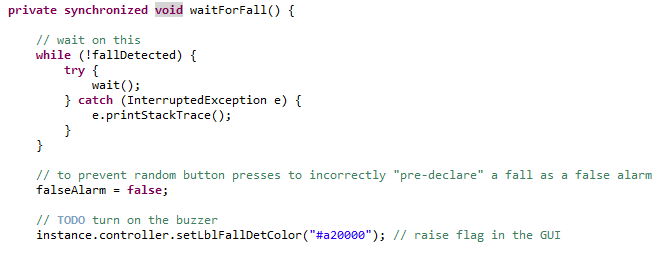
\includegraphics[scale=0.80]{images/UI_2.png}
	\caption{waitForFall method}
	\label{img:UI_2}
\end{figure}
\FloatBarrier

Then if a False Alarm happens, the color of the "Help Requested" label remains black, else it changes to red.
\FloatBarrier
\begin{figure}[h]
	\centering
	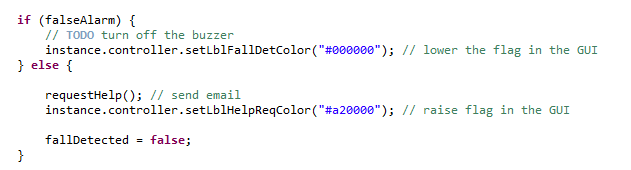
\includegraphics[scale=0.80]{images/UI_3.png}
	\caption{False Alarm}
	\label{img:UI_3}
\end{figure}
\FloatBarrier

\vskip 1cm
\subsection{UI Graphs}
Since our User Interface will feature graphs for both the Accelerometer as well as the Gyroscope data, we implemented two LineCharts in the main menu of the UI. The idea is to use series, which are imported using the XYChart JavaFX class. After receiving the data directly from the methods in the Mathematics class that the team implemented, the functions will assign the data to these series and then visualize it, by adding it to the respective LineChart.
\\\\Since a single LineChart can handle multiple series, and since we have two Sensortags that will be connected at once, each graph will feature two series, which equals to four series total. The data is passed to these series using four queues. When a series reaches the maximum number of allowed data, it is updated in the same way a queue is in that the first element in gets removed from the graph, and the new element is pushed on top. This will be updated in real time.\\
As of the point this report was written, the method is yet to be tested. For testing the real time updating visuals, we will populate the queues with random numbers from the existing Java class Math.

\section{Adapting the Math Model}
While it is still not possible to test the actual values received by the Sensortags, we can still change the code to better fit with the rest of the application. Since the format of the input, which is at the same time the output of the Sensortags, is known, the methods were changed to accept that data and use it.\\\\
At the same time, we must concern ourselves with the output of the Math model, and how it will fit into the User Interface. So far, the accelerometer readings from both Sensortags will be passed on either as singular absolute values, or queues of absolute values that have a certain specified size. The slightly more difficult part is adapting the output of the gyroscopes, as each sensor has three values of X, Y, and Z, the values of which vary greatly and are difficult normally to represent in a graph.\\
As a result, a decision was made to turn these values into angles, which would mean that the possible variance becomes from the value 0 to 360. This fixes the problem, as it simultaneously allows the data to be more easily graphed without actually affecting the fall detection algorithm itself. 

\section{Measurement Chain\textsuperscript{\cite{prodspec}}}
For our application we make use only of the MPU-9250 sensor pack, which includes a three-axis accelerometer, a three-axis gyroscope and a three-axis magnetometer (the last is not used and was deactivated).\\\\
The measuring object is the sensor itself (the acceleration and orientation of it). Since it is rigidly mounted on the PCB, we can assume that corresponds to measuring the movement of the whole Sensortag. However, we cannot ignore the soft connection of the Sensortag to the belt and of the belt to the user. This would require adaptation of the fall detection algorithms to many different user/clothing combinations.\\
The measured quantities are: the total resulting acceleration (gravity plus motion); and angular velocity.\\
The measurement method is indirect (see individual sensor description below).\\\\
The complete measurement chain consists of the sensors themselves, the ADCs built into the MPU-9250, and the number conversion that takes place in the desktop part of the application. Since the signals are transmitted only after the analog to digital conversion takes place, we don’t have to worry about transmission induced errors.

\subsection{Accelerometer}
"The accelerometer uses separate proof masses for each axis. Acceleration along a particular axis induces displacement on the corresponding proof mass, and capacitive sensors detect the displacement differentially." The analog value is digitalized by three 16bit sigma-delta ADC (one per axis). The resulting value may be written as:
$$ a = val \pm e_i \pm e_T \pm e_l \pm e_{cal} \pm e_n \quad g $$
Where val is the real value, $e_i$ is the intrinsic error (3\%), $e_T$ is the temperature induced error (0.026\%/$^{\circ}$C), $e_l$ is the non-linearity error (0.5\%), $e_{cal}$ is the initial calibration error (80 mG) and $e_n$ is the noise (8 mG). At room temperature and for the threshold values used by our fall detection algorithm, the above formula can be approximated with:
$$ a = val \pm 6\%  \quad g $$

\subsection{Gyroscope}
The gyroscope’s sensors consist of 3 vibratory MEMS. "When the gyros are rotated about any of the sense axes, the Coriolis Effect causes a vibration that is detected by a capacitive pickoff." The resulting value may be written as:
$$ v_{ang} = val \pm e_i  \pm e_T \pm e_l \pm e_{cal} \pm e_n \quad ^{\circ}/s $$
Where val is the real value, $e_i$ is the intrinsic error (3\%), $e_T$ is the temperature induced error (4\%), $e_l$ is the non-linearity error (0.1\%), $e_{cal}$ is the initial calibration error (5 $^{\circ}/s$) and $e_n$ is the noise (0.1 °/s). At room temperature and for the threshold values used by our fall detection algorithm, the above formula can be approximated with:
$$ v_{ang} = val \pm 9\% \quad ^{\circ}/s $$
\\\\

\section{Effort Hours}
\begin{itemize}
	\item \textbf{Raul Bertone:} 15h
	\item \textbf{Elis Harruni:} 21h
	\item \textbf{Muyassar Kokhkharova:} 8h
	\item \textbf{Saidar Ramazanov:} 11h
	\item \textbf{Xhoni Robo:} 22h
\end{itemize}

\textbf{Total Effort}: 77h\\\\
\clearpage
%----------------------------------------------------------------------------
% Bibliography
%----------------------------------------------------------------------------	
\printbibliography
\end{document}
%----------------------------------------------------------------------------
